\documentclass[twoside]{article}
\usepackage{package}
\usepackage[T1]{fontenc}
\usepackage{subfiles}
% Silenciar la advertencia de versalita + negrita inexistente
\WarningFilter{latex}{Some font shapes were not available}
\WarningFilter{latex}{Font shape `T1/lmr/bx/sc'}

% Silenciar la advertencia de caracteres perdidos en el nullfont (para 01_introduccion.tex)
\WarningFilter{latex}{Missing character: There is no}
%Nuevos comandos
\renewcommand{\thefootnote}{\arabic{footnote}}
\raggedbottom



\begin{document}
\begin{center}
    \thispagestyle{empty}
    \large{\textsc{Matrices en MATLAB y Respuesta Transitoria}}\\[0.5cm] 
    \large{Fabrizio Benavidez\footnote[1]{\texttt{fabrizio.benavidez@mi.unc.edu.ar}}}\\[0.5cm]

    \large{\footnotemark[1]\textit{Facultad de Ciencias Exactas, Físicas y Naturales, Ingeniería Aeronáutica}}
    \\[0.5cm]

    \begin{minipage}{0.7\textwidth}
    \hrule
    \vspace{0.2cm}
        \normalsize{\textsc{Resumen} En el siguiente trabajo se realiza código MATLAB para calcular el lugar de raíces para distintos tipos de sistemas, así como funciones de lazo cerrado. Además, se trabaja por primera vez con funciones: fragmentos de código que se pueden declarar las veces necesarias. Se crean dos tipos de funciones: uno para calcular raíces cuadradas y otras para calcular factor de amortiguamiento, frecuencia y ganancia.}\\[0.2cm]
        \normalsize{\textit{Palabras claves}: lugar de raíces, compensadores, funciones \ }
    \vspace{0.2cm}
    \hrule
    \end{minipage}
    
    \vfil

    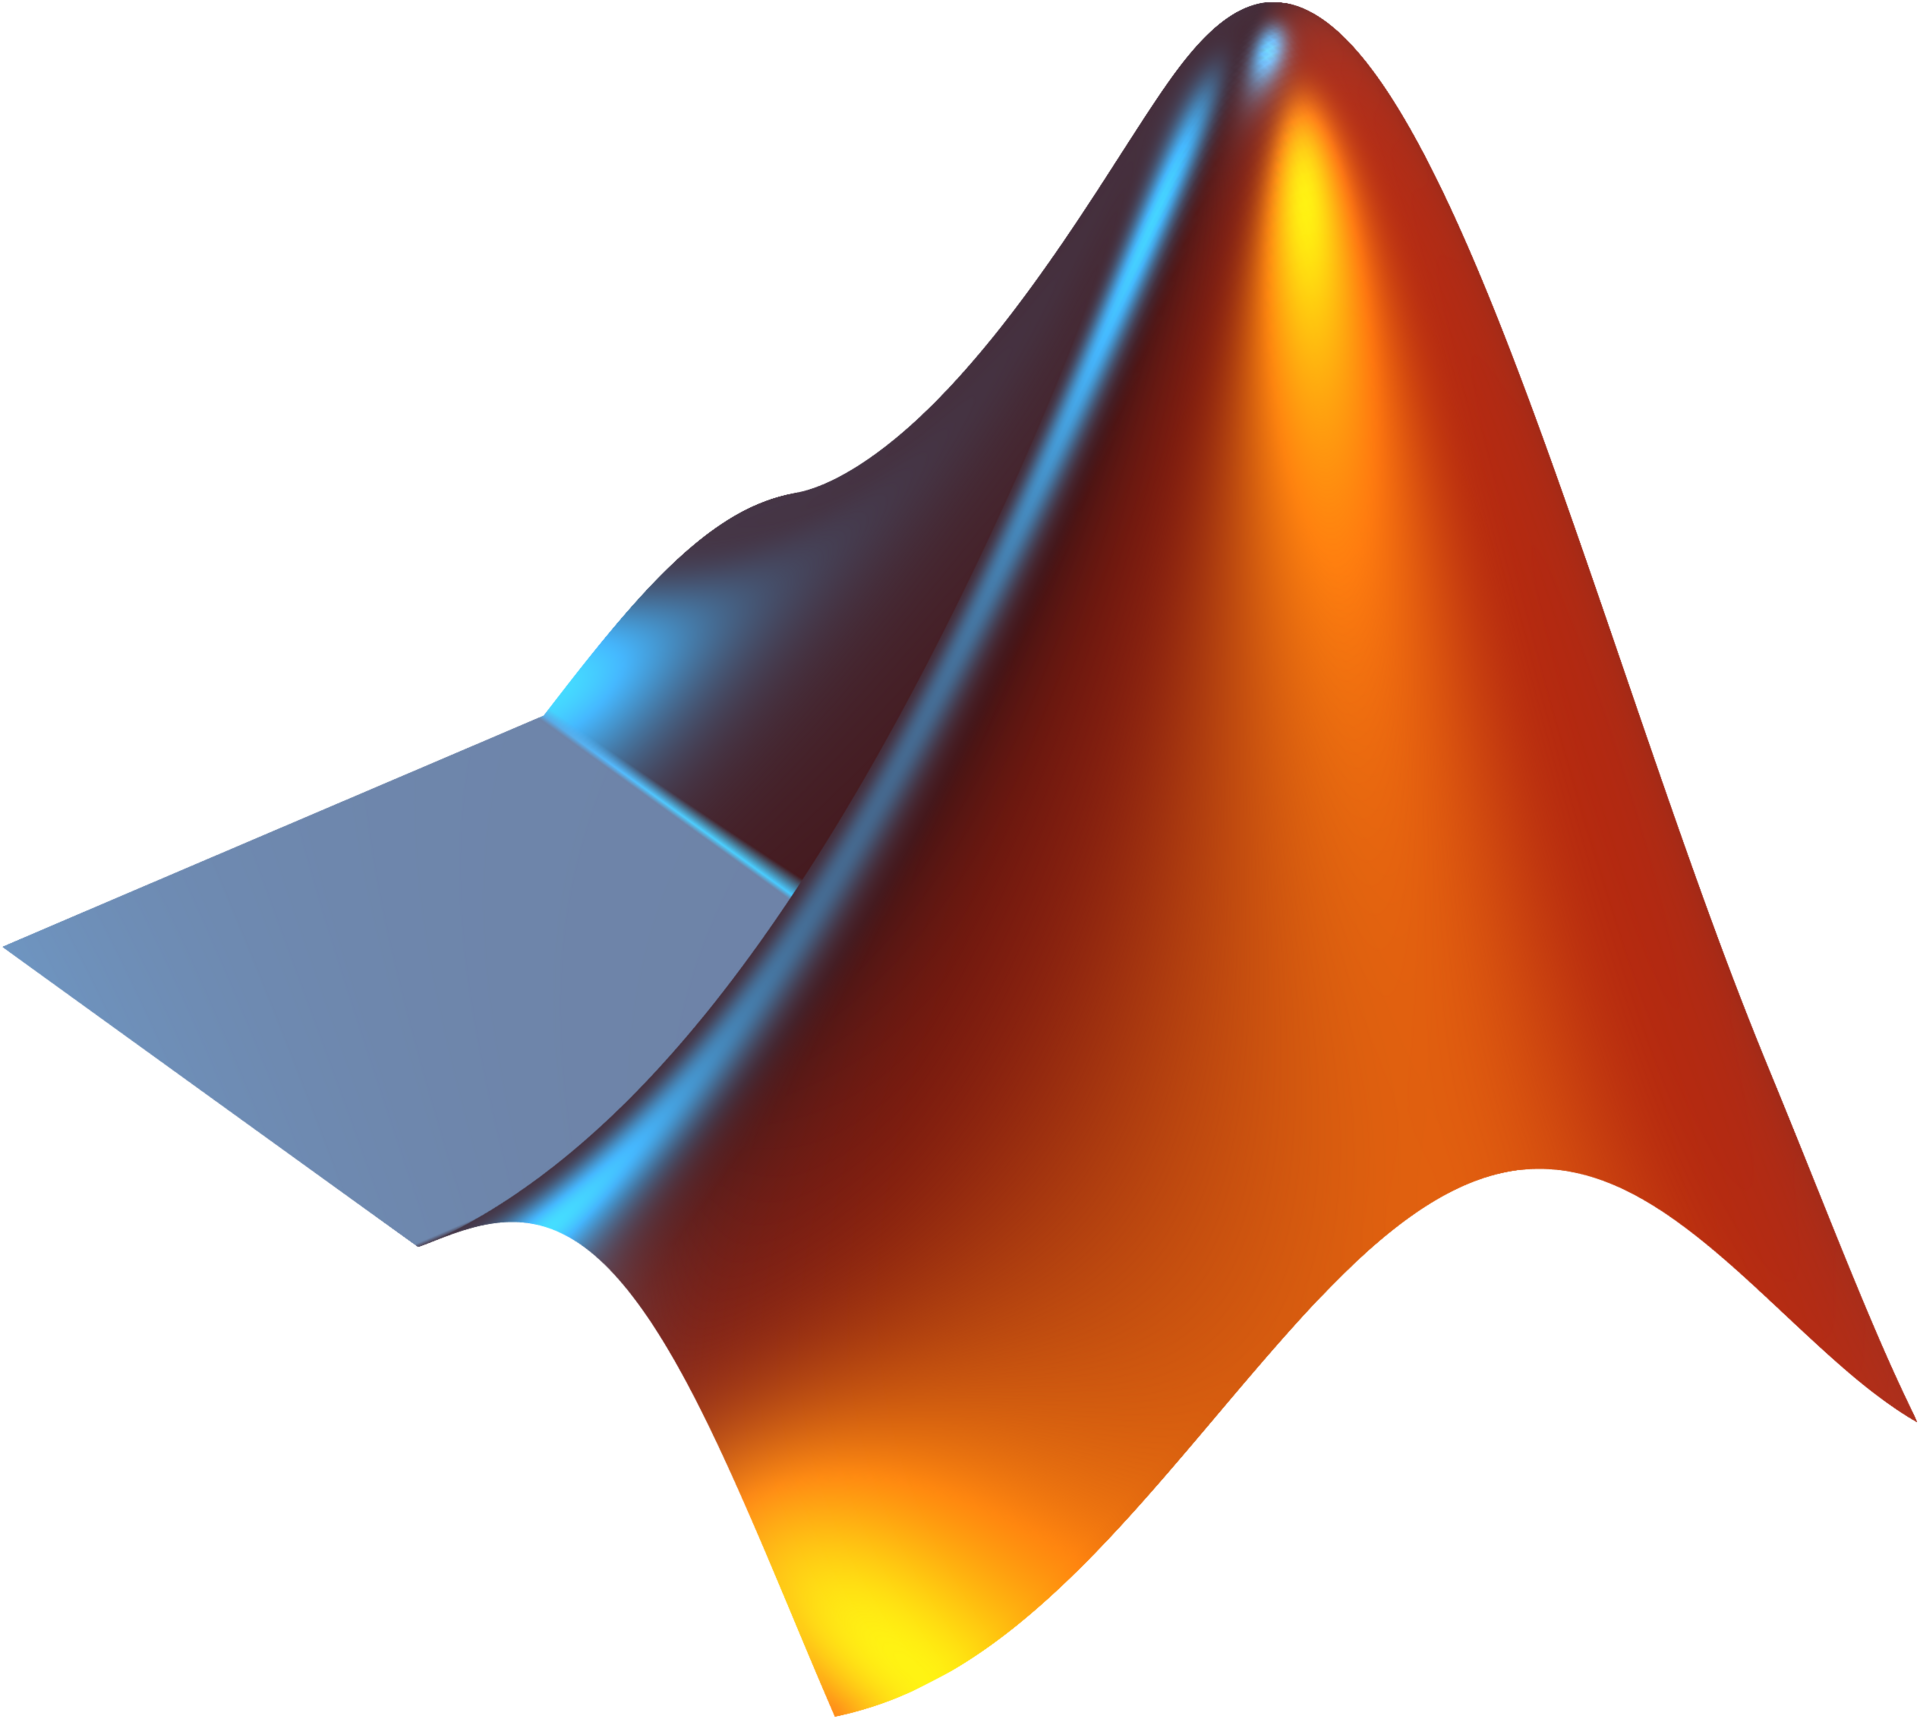
\includegraphics[width = 0.4\textwidth]{imagenes/Matlab_Logo.png}\\[0.5cm]

    \vfil

    \today\\[0.2cm]
    \large{Semana 6}
\end{center}





\newpage

\section*{Guía 11: Compensadores proporcionales} 
\subfile{secciones/guia11}

\newpage

\section*{Guía 12: Funciones en MATLAB} 
\subfile{secciones/guia12}














\newpage
% \thispagestyle{empty}
% \bibliography{biblioteca.bib}
% \bibliographystyle{plain}


\end{document}